	% %%%%%%%%%%%%%%%%%%%%%%%%%%%%%%%%%%%%
% A LaTeX template for the technical essay of TTM4137 Wireless Security
% Stig F. Mjolsnes, 01.09.2012
%%%%%%%%%%%%%%%%%%%%%%%%%%%%%%%%%%%%%
\documentclass[a4paper,11pt]{article}

\usepackage[plain]{fullpage}
\usepackage{graphicx}  %This enables the inclusion of pdf graphic files in figures
\usepackage{hyperref} % Make links in your document click-able NB: must be loaded before the caption-package
\usepackage{caption}
\usepackage{subcaption}
\usepackage{wrapfig}
\usepackage{sidecap}
\usepackage[utf8]{inputenc}


\title{Attacks on Near Field Communications on Mobile Phones}
\author{Håkon Nymo Matland \\
	\texttt{hakonnym@stud.ntnu.no}\\
	TTM4137 Wireless Security Technical Essay}
\date{\today}

\begin{document}
\maketitle


\section{Introduction}
The Near Field Communication (NFC) technology is being deployed in mobile phones all over the world. The technology's applications is wide~\cite{remedios2006nfc}. Several companies focus on one of it's most promising applications: payment solutions using NFC~\cite{tan2013}. An analysis by Berg Insight claim that one in three mobile phones will come with NFC by 2017~\cite{nfc_growth}, making the technology a huge future marked.

\paragraph{}NFC is a set of standards for devices to establish radio communication with each other by bringing them in close proximity, usually not more then a few centimeters. The standards are based on RFID, and mixed with other standards cover data exchange formats and communication protocols. Communication is possible between two NFC enabled devices, or a NFC enabled device and unpowered NFC chip.

\paragraph{}The need of security and robustness is very important, as an insecure and attackable device would give criminals new ways to steal funds, or simply take control over the device. Different attacks have been proven successful and malicious, and the threat should be taken seriously by both individuals and corporations. Simple RFID-stickers and vulnerabilities in software is all an attacker need to do harm. This essay will present and discuss some of the successful attacks previously demonstrated by experts in the field of NFC and security.


\section{Threats on NFC enables devices}
\begin{wrapfigure}[10]{R}{0.45\textwidth}
  \centering
  \vspace{-2cm}
  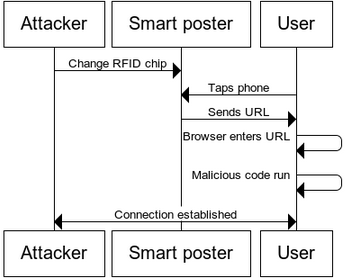
\includegraphics[scale=0.6]{SD_SmartPoster1} %Note: no use of .jpg file ending
  \vspace{-0.7cm}
  \caption{Possible smart poster attack
  \label{fig:SD_SmartPoster1}}
\end{wrapfigure}
\subsection{Smart poster URI spoofing}

With the deployment of NFC capable mobile phone, the concept of smart posters came.
The poster is used to advertise or give the customer a service. The user only has to tap their NFC enabled mobile phone in close proximity to the advertisement, and something happens on the phone~\cite{ruiz2009university}~\cite{smartposter}. Through social engineering or software vulnerabilities this can be exploited. Changing the RFID chip in the poster makes it possible for customers to believe they are accessing a legitimate service, while they are not.

\subsubsection{Web browser exploits}

A possible scenario is an user tapping their phone on a smart poster to gain the URL of a service. If an attacker has changed the RFID chip to one of his own, he can trick the users to enter a spoofed URL, with the goal of phishing sensitive information through a login or sign up form. 

In 2012 security researcher Charlie Miller proved how he with a simple RFID sticker could gain full root shell access on an Android phone~\cite{cmiller}~\cite{cmiller1}. With full root shell acces, several exploits are possible. Charlie miller was able to download every file on the  Although the attack primarily used exploitable bugs in the browser, the attack was triggered by the mobile phones NFC.

\subsubsection{Malicious software download}
The concept described in the previous section can also be used more explicitly to run malicious code on the device. The attacker has the possibility to trick the user into downloading an application to install directly. On Android devices you could simply use the smart poster to direct the user to a .apk file on the internet. If the poster is trying to advertise an app, a user not thinking critically might install the application, and make the device send all kind of data to the attacker.

\subsubsection{Premium rated telephone services}

Similar to have a RFID chip send a web URL, it can also be used to invoke telephone connections or sending sms~\cite{mulliner2009vulnerability}. The user might be asked if he wants to call or send, but some users will likely not pay attention to what is says on the screen if it is received from what looks to be a legitimate source. This opens a whole new range of premium service rate scams. A poster claiming to let you call a free service might suddenly make an user call an expensive premium rate number. A user trying to purchase something from a vending machine might end up with a high phone bill, and no snack.

\subsection{Eavesdropping}
As with every other wireless communication interface eavesdropping is an obvious threat. If the communication is not properly encrypted and secured, parties not participating in the transmission of data may capture the radio frequencies and store them for analysis. An experiment as part of the master thesis by Henning Siitonen Kortvedt at the Norwegian University of Science and Technology concluded that it is practical possible to capture and demodulate data sent in both directions between two NFC devices~\cite{kortvedt2009eavesdropping}~\cite{kortvedt2009securing}.


\subsection{Denial-of-Service attacks}
A Denial-of-service attack(DoS attack) is an attempt to make a service unavailable to its intended users. The motivation for an attacker to perform a DoS attack may vary, but the result is nonetheless destructive. DoS attacks may be used to destroy the trust relationship between the customer and the service provider.
\subsection{Requirements of Form}


\section{Conclusion}


\begin{figure}[hbp]
	\centering
	\begin{subfigure}[b]{0.3\textwidth}
		\centering
		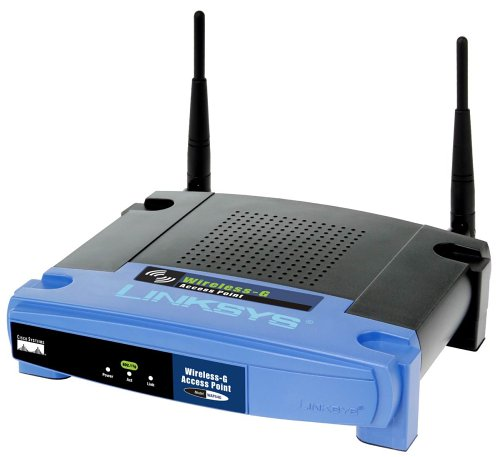
\includegraphics[scale=0.20]{linksys}
		\caption{Scale=0.20}
	\end{subfigure}
	\begin{subfigure}[b]{0.3\textwidth}
		\centering		
		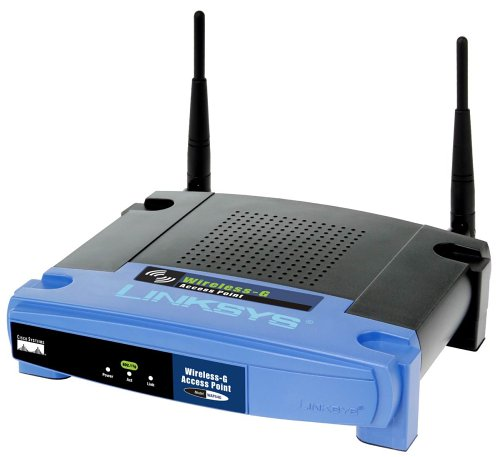
\includegraphics[scale=0.15]{linksys}
		\caption{Scale=0.15}	
	\end{subfigure}
	\begin{subfigure}[b]{0.3\textwidth}
		\centering		
		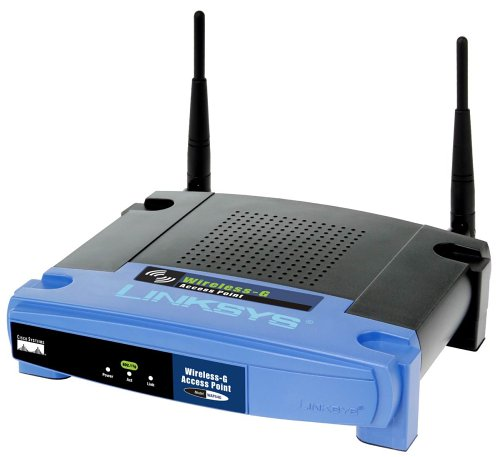
\includegraphics[scale=0.10]{linksys}
		\caption{Scale=0.10}
	\end{subfigure}
	\caption{The Linksys WRT54G line of routers include both  802.3 Ethernet and 802.11b/g wireless LAN.}
	\label{fig:linksys}
\end{figure}

% It is highly recommended to keep your references in a separate file (here called "references.bib")
% However if you want to create the reference section manually, 
% uncomment the lines below starting at "\begin{thebibliography} ... etc"
\bibliographystyle{unsrt}
\bibliography{references}\label{sec:references}



%\begin{thebibliography}{N}\label{sec:references}
%\bibitem{wiki1} Wikipedia. \textit{Citation.} Available at \url{http://en.wikipedia.org/wiki/Citation}.
%
%\bibitem{Daborn} Gordon Baxter, Jon Lewis and Ishbel Duncan. \textit{What is a Technical Essay?}
%Available online at \url{http://ishbel.host.cs.st-andrews.ac.uk/WhatisaTechnicalEssay.pdf}.
%
%\bibitem{Kortvedt} Henning Kortvedt and Stig Frode Mj{\o}lsnes. \textit{Eavesdropping Near Field Communication}.  
%In The Norwegian Information Security Conference (NISK 2009) Proceedings, pp. 57-68.  Tapir Akademiske Forlag, 2009.
%
%\end{thebibliography}  


\end{document} 
